\documentclass[parskip]{scrartcl}
\usepackage[utf8]{inputenc}
\usepackage[ngerman]{babel}
\usepackage[round]{natbib}
\usepackage{color} % used for comments
\usepackage{listings}
\usepackage{url}
\usepackage{graphicx}
\usepackage[hidelinks]{hyperref}
\usepackage{float}
\usepackage{array}
\usepackage{longtable}
\newcolumntype{L}[1]{>{\raggedright\let\newline\\\arraybackslash\hspace{0pt}}m{#1}}
\newcolumntype{C}[1]{>{\centering\let\newline\\\arraybackslash\hspace{0pt}}m{#1}}
\newcolumntype{R}[1]{>{\raggedleft\let\newline\\\arraybackslash\hspace{0pt}}m{#1}}
\graphicspath{ {img/} }
\lstset {
  language=xml,
  basicstyle={\footnotesize\ttfamily},
  numbers=none,
  aboveskip=5mm,
  belowskip=5mm,
  showstringspaces=false,
  columns=flexible,
  keywordstyle={\bfseries\color{blue}},
  commentstyle={\color{red}\textit},
  stringstyle=\color{magenta},
  frame=single,
  breaklines=true,
  breakatwhitespace=true,
  tabsize=4,
  morekeywords={rdf,rdfs,owl}  % <-- adding custom keywords
}

% \linespread{1.2}

\begin{document}
\subject{Projektdokumentation im Modul Semantic Web}
\title{Verbreitung von Musiktiteln nach deren Verwendung in einem Kinofilm}
\author{Patrick Bachmann}
\date{\today}

\maketitle


\paragraph{Recherchefragestellung: }
Welche Musiktitel sind nach der Verwendung in einem Kinofilm in den Top 50 der Charts aufgetaucht?

\section{Inhaltliche Interpretation der Fragestellung}

Die Verwendung von Musik in Filmen ist ein gängiges Mittel um den gezeigten Bildern mehr Ausdruck zu verleihen und die Stimmung hervorzuheben. Neben der klassischen Filmmusik, welche individuell für den Film angefertigt wird, werden auch häufig kommerzielle Titel von Künstlern verschiedenster Stilrichtungen und Bekanntheitsgrade verwendet.

Die Fragestellung soll untersuchen, welche kommerziellen Musiktitel nach der Verwendung in einem Kinofilm populär wurden bzw. erneut Popularität erreichten.

\pagebreak
\section{Relevante Datenquellen}

Für die Beantwortungen der Fragestellung werden folgende Daten benötigt:
\begin{itemize}
    \itemsep 1pt
    \parskip 0pt
    \parsep 0pt
    \item Kinofilme
    \begin{itemize}
            \item enthaltene Musiktitel
            \item Veröffentlichungsdatum
    \end{itemize}
        \item Charts
\end{itemize}

Nachfolgend sind die Datenquellen aufgelistet, welche benutzt wurden um diese Informationen zu akquirieren.

\subsection{Tunefind}
\label{subsec:tunefind}

Tunefind ist eine Community geführte Datenbank für Musiktitel, welche in Serien und Kinofilmen Verwendung fanden.

\begin{tabular}{l|p{9cm}}
	Link & \url{http://www.tunefind.com/} \\
 	Datenformat & JSON \\
 	Schnittstelle & REST-Api \\
 	Lizenz & siehe \url{http://www.tunefind.com/api} \\
 	Open Data & $\star\star\star$ \\
\end{tabular}

\subsection{OMDb - The Open Movie Database}

Die Open Movie Database ist eine Web-Service, welcher eine Auswahl an Daten der IMDB über eine API zur Verfügung stellt. Es ist möglich einen Film über seinen  Titel oder seine IMDb ID zu finden. Die Suche über den Titel funktioniert dabei wie eine typische Suchfunktion und liefert auch bei verschiedenen Schreibweisen des Titels zuverlässig Ergebnisse.

\begin{tabular}{l|p{9cm}}
    Link & \url{http://www.omdbapi.com/} \\
    Datenformat & JSON, XML \\
    Schnittstelle & REST-API \\
    Lizenz & unbekannt \\
    Open Data & $\star\star\star$ \\
\end{tabular}

\subsection{IMDb}

Die Internet Movie Database ist die größte Datenbank für Filme, Serien und Spiele. Sie enthält eine Vielzahl von Informationen wie z.B. Regisseur, Schauspieler und die Veröffentlichungsdaten getrennt nach Ländern.

\begin{tabular}{l|p{9cm}}
	Link & \url{http://www.imdb.com/} \\
 	Datenformat & HTML \\
 	Schnittstelle & HTTP \\
 	Lizenz & unbekannt \\
 	Open Data & $\star\star$ \\
\end{tabular}

\subsection{Offizielle Charts}

Die Offiziellen Charts werden von der GfK zur Verfügung gestellt. Seit dem 02.01.1978 werden hier wöchentlich die Verkaufszahlen von Musik in Deutschland mit einem Ranking von 1 bis 100 bewertet. Dabei gilt es verschiedene Unterteilungen wie z.B. Single, Album und Compilation.

\begin{tabular}{l|p{9cm}}
    Link & \url{https://www.offiziellecharts.de} \\
    Datenformat & HTML \\
    Schnittstelle & HTTP \\
    Lizenz & unbekannt \\
    Open Data & $\star\star$ \\
\end{tabular}

\section{Extraktion relevanter Daten und import in einen Triplestore }

Die Extraktion der Daten wurde bei allen Datenquellen über Python-Skripte realisiert. Für jede Datenquelle wurde ein Skript mit zwei Phasen erstellt. Die \texttt{LoadFromWeb}-Phase lädt die Daten von der Datenquelle herunter und speichert sie als Textdatei mit JSON-Format ab. Die \texttt{ConvertToRdf}-Phase lädt die abgespeicherten Daten aus der vorher gespeicherten Datei und wandelt diese in Tripel um, welche im Turtle-Format abgespeichert werden. Die Phasen können kombiniert oder einzeln ausgeführt werden. Dafür muss dem Skript das Argument \texttt{-l} für die \texttt{LoadFromWeb}-Phase und \texttt{-r} für die \texttt{ConvertToRdf}-Phase mitgegeben werden.

Die erzeugten Dateien werden im Ordner \texttt{data/} abgelegt. Die Dateinamen sind im Kopfbereich des jeweiligen Skriptes festgeschrieben.


\subsection{Verwendete Bibliotheken}

\paragraph{HTML Extraktion}
Für die Extraktion von Daten aus HTML-Dateien wird die Bibliothek \texttt{beautifulsoup4  (v4.3.2)}\footnote{\href{http://www.crummy.com/software/BeautifulSoup/}{http://www.crummy.com/software/BeautifulSoup/}} verwendet. Sie ermöglicht ein einfaches arbeiten auf dem DOM-Baum.

\paragraph{RDF}
Für das Erstellen der Tripel sowie die Speicherung im Turtle-Format wird \texttt{rdflib (v4.2.0)}\footnote{\href{https://github.com/RDFLib/rdflib}{https://github.com/RDFLib/rdflib}} verwendet. 

\subsection{Extraktion Tunefind}

Tunefind stellt eine API bereit, welche die Daten der Webseite im JSON- oder XML-Format abrufbar macht. Für die Benutzung der API war eine Registrierung erforderlich. Anschließend konnte ein API Benutzernamen und ein API Passwort angefordert werden.
Um den Endpunkt von Tunefind erfolgreich anzusprechen, mussten einige Besonderheiten bzgl. des HTTP-Request-Headers beachtet werden. \autoref{lst:httpHeader} zeigt den verwendeten Header.

\begin{lstlisting}[caption={HTTP-Request-Header}, label={lst:httpHeader}]
accept: "text/html, application/json"
accept-encoding: "gzip, deflate"
authorization: "Basic %login%"
user-agent: "%appName%;%email%"
\end{lstlisting}

\begin{description}
    \item[accept] \hfill \\
        Gibt das erwartete Antwortformat an. Da JSON sich sehr gut mit Python verarbeiten lässt, wurde dieses Format gewählt.
    \item[accept-encoding] \hfill \\
        Gibt an, dass die Daten gzip-komprimiert erwartet werden.
    \item[authorization] \hfill \\
        Angaber der API-Login Daten für die HTTP-Basic-Authentication.
        Die Variable \texttt{\%login\%} wird mit dem base64-codierten Login-String bestehend aus API Benutzernamen und API Passwort ersetzt.
    \item[user-agent] \hfill \\
        Gibt an, welche Anwendung die Anfrage abgeschickt hat. Der Endpunkt von Tunefind lehnt jede Anfrage ab, welche diese Eigenschaft nicht mitschickt. Da es zum guten Ton gehört, wurde neben dem Anwendungsnamen auch eine E-Mail Adresse für die Kontaktaufnahme angegeben.
\end{description}

Weiterhin ist der Endpunkt auf eine Anfrage pro Sekunde limitiert.

Die \texttt{LoadFromWeb}-Phase und somit die Durchführung der Datenakquise beginnt mit einer Anfrage an:\\
\texttt{https://www.tunefind.com/api/v1/movie}

Das Ergebnis ist eine Liste mit allen in der Datenbank vorhandenen Filmen. Über die erhaltene ID können nun die Details zu jedem Film abgerufen werden. Dies geschieht mit Anfragen an:\\
\texttt{https://www.tunefind.com/api/v1/movie/<movie-id>}

Diese Details enthalten unter anderem die Musiktitel, welche zu dem ausgewählten Film in der Datenbank hinterlegt sind.
Mit diesen Daten wird eine Liste mit allen verfügbaren Filmen und ihren Musiktiteln erstellt. \autoref{lst:tunefindJson} zeigt das JSON-Format, in welchem das dabei entstandene Ergebnis abgespeichert wird.

\begin{lstlisting}[caption={Tunefind JSON-Format}, label={lst:tunefindJson}]
[  
    {  
        "soundtrack":[  
            {
                "artist": "",
                "title": ""
            },
        ...
        ],
        "title": ""
    },
    ...
]
\end{lstlisting}

Die \texttt{ConvertToRdf}-Phase lädt die abgespeicherten Daten wieder und konvertiert sie in Tripel. Das dazu verwendete Schema zeigt \autoref{fig:tunefindrdf}.

\begin{figure}[H]
    \centering
    \caption{Tunefind RDF Schema}
    \label{fig:tunefindrdf}
    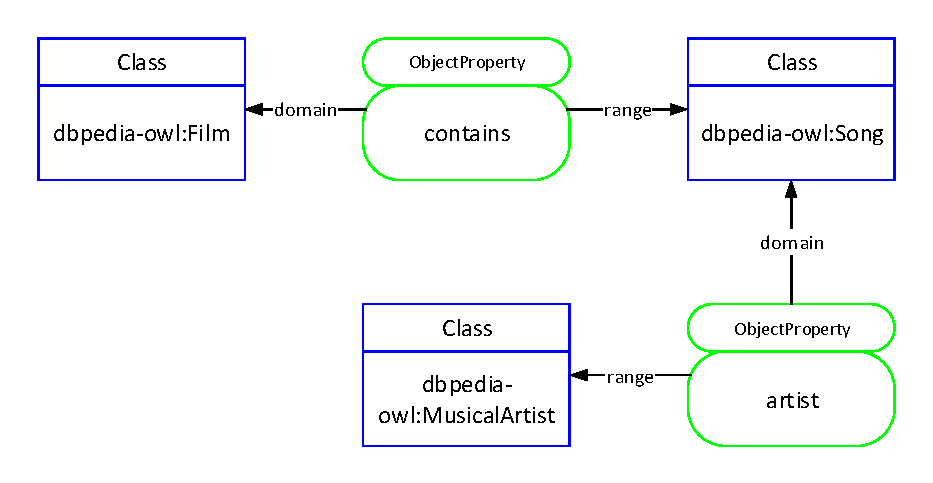
\includegraphics[scale=0.8]{tunefind}
\end{figure}
\subsection{Extraktion OMDb}

Das OMDb Projekt stellt über eine API Daten der IMDb bereit, da diese selbst keinen Endpunkt zur Verfügung stellt. Der Endpunkt der OMDb ist frei benutzbar und erfordert weder eine Registrierung noch einen API-Schlüssel.

Die OMDb wird als Zwischenschritt für die Extraktion der Daten von der IMDb (siehe \ref{subsec:imdb}) genutzt. Der zur Verfügung gestellte Endpunkt verfügt über eine Möglichkeit zur Volltextsuche nach Filmtiteln. Diese wird genutzt um zu den Filmtiteln von Tunefind die entsprechenden IMDb Datensätze finden. Dazu wird mit den jedem Filmtitel folgende URL aufgerufen\\
\texttt{http://www.omdbapi.com/?t=<Filmtitel>\&plot=short\&r=json}

Als Ergebnis werden die wichtigsten Informationen über den angegebenen Film zurück--geliefert. Darunter ist auch die ID des Films in der IMDb. \autoref{lst:omdbJson} zeigt das JSON-Format, in welchem der Filmtitel von Tunefind und die IMDb ID abgespeichert werden.

\begin{lstlisting}[caption={OMDb JSON-Format}, label={lst:omdbJson}]
[  
    {  
        "title": ""
        "imdbid": ""
    },
    ...
]
\end{lstlisting}

Eine Konvertierung in Tripel ist bei dieser Datenquelle nicht nötigt, da sie nur als Zwischenschritt zur Gewinnung der IMDb ID dient.

\subsection{Extraktion IMDb}
\label{subsec:imdb}

Die IMDb als größte Film- und Fernseh-Datenbank stellt von sich aus keinen Endpunkt zur Verfügung. Weshalb die benötigten Daten aus den HTML-Seiten extrahiert werden müssen. Mithilfe der ID, welche über die OMDb gewonnen wurde, kann nun für jeden Film die entsprechende Unterseite in der IMDb aufgerufen werden.

Die Veröffentlichungsdaten werden der \textit{ReleaseInfo}-Seite für den jeweiligen Film entnommen:\\
\texttt{http://www.imdb.com/title/<ID>/releaseinfo}

Weiterhin werden die Schauspieler und Regisseure aus der \textit{Credit}-Übersicht des Films extrahiert:\\
\texttt{http://www.imdb.com/title/<ID>/fullcredits}

Die Speicherung der extrahierten Daten erfolgt erneut im JSON-Format. Für den Filmtitel wird dabei statt dem in der IMDb hinterlegten Titel der Titel von Tunefind benutzt. Dies ermöglicht bei der späteren Verlinkung der Ressourcen ein einfaches Zuordnen der Daten. \autoref{lst:imdbJson} zeigt das JSON-Format, in welchem die Daten abgespeichert werden.

\begin{lstlisting}[caption={IMDb JSON-Format}, label={lst:imdbJson}]
[  
    {  
        "directors":[  
            "",
            ...
        ],
        "cast":[
            {
                "name": "",
                "screen_name": ""
            }
            ...,
        ],
        "release_info":[
            {
                "country": "",
                "event": "",
                "date": ""
            }
            ...,
        ],
        "title": "",
        "imdbID": ""
    },
    ...
]
\end{lstlisting}

In der Konvertierungs-Phase wurden nachträglich Einschränkungen hinzugefügt, um die Anzahl der erzeugten Tripel zu verringern (siehe \ref{subsec:problems}). Es werden nur Filme übernommen, deren frühstes Veröffentlichungsdatum mindestens im Jahr 2005 liegt. Weiterhin werden nur die Veröffentlichungsdaten von Deutschland, Großbritannien sowie den USA und die ersten zehn Schauspieler konvertiert. Die Regisseure werden uneingeschränkt übernommen. Das dazu verwendete Schema zeigt \autoref{fig:imdbrdf}.

\begin{figure}[H]
    \centering
    \caption{IMDb RDF Schema}
    \label{fig:imdbrdf}
    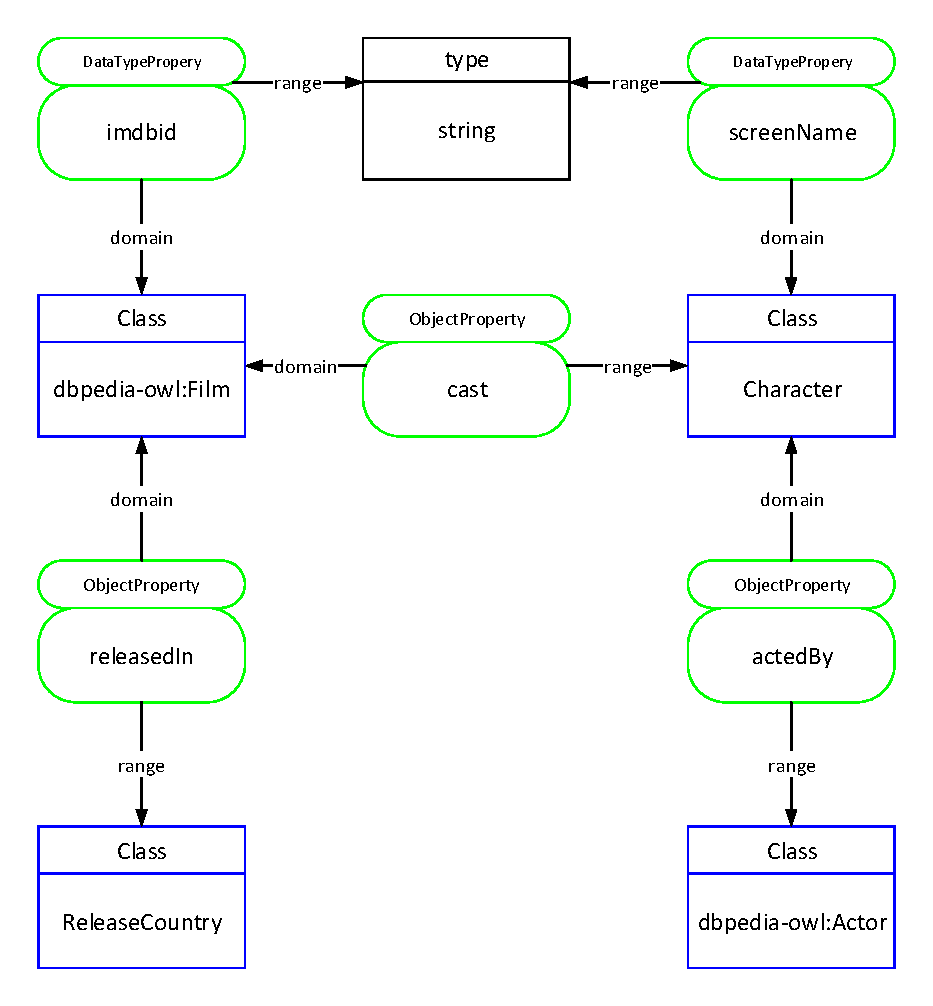
\includegraphics[scale=0.8]{imdb}
\end{figure}

\subsection{Extraktion Charts}

Wie auch die IMDb, stellen die Offiziellen Charts keine API zur Verfügung. Weshalb auch hier auf die Daten aus den HTML-Seiten zurückgegriffen werden muss.

Die Akquirierung der Daten erfolgt in einem Zeitraum vom 01.01.2000 bis zum 31.05. 2015. Es wird mit einem Intervall von sieben Tagen gearbeitet, da die Charts nur wöchentlich aktualisiert werden. Für den Aufruf der folgenden URL muss das Datum in Millisekunden umgerechnet und an die Stelle \texttt{<date>} eingesetzt werden:\\
\texttt{https://www.offiziellecharts.de/charts/single/for-date-<date>}

Die Extraktion der Daten wird auf die ersten 50 Chart-Einträge jeder Woche begrenzt. \autoref{lst:chartsDeJson} zeigt das JSON-Format, in welchem die Daten abgespeichert werden.

\begin{lstlisting}[caption={Offizielle Charts JSON-Format}, label={lst:chartsDeJson}]
[  
    {
        "tracks": [
            {
                "artist": "",
                "title": "",
                "pos": ""
            }
            ...,
        ]
        "date": ""
    },
    ...
]
\end{lstlisting}

Wie auch bei der IMDb wurden nachträglich Einschränkungen zur Konvertierungs-Phase hinzugefügt, um die Anzahl der Tripel zu verringern. Entsprechend der Einschränkung bei der IMDb, werden nur Charts ab dem 01.01.2005 konvertiert. Das dazu verwendete Schema zeigt \autoref{fig:chartrdf}.

\begin{figure}[H]
    \centering
    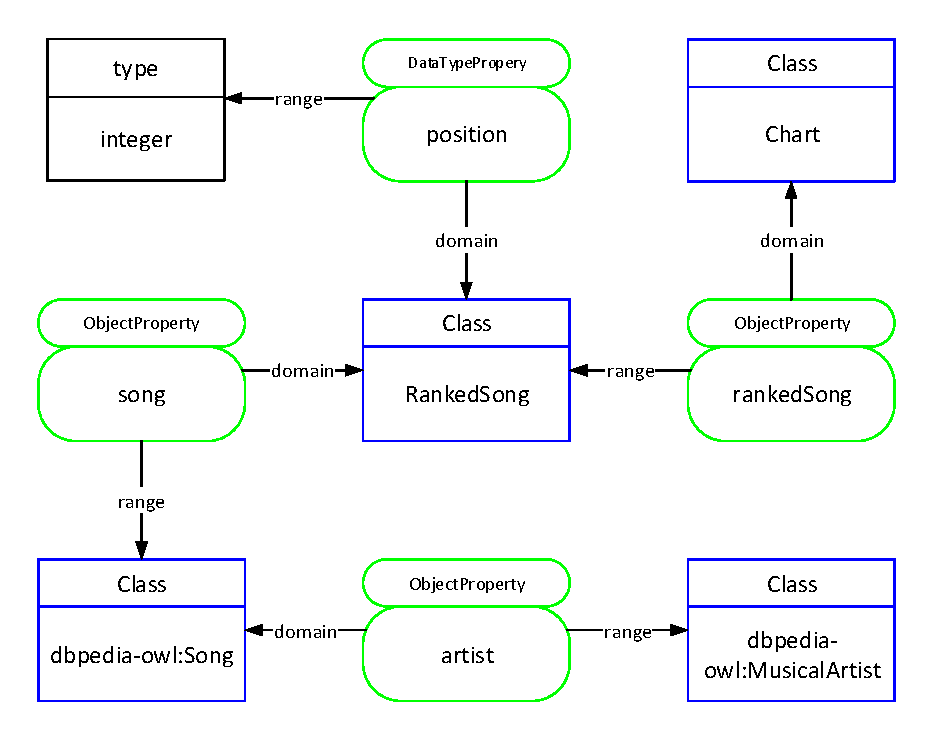
\includegraphics[scale=0.8]{charts}
    \caption{Charts RDF Schema}
    \label{fig:chartrdf}
\end{figure}

\subsection{Import in einen Triplestore}
Als Triplestore wurde Stardog\footnote{\url{http://www.stardog.com}} in der Community Edition verwendet. Er zeichnet sich durch eine einfache Handhabung und Konfiguration aus.

Es wurde versucht den Import der Tripel über die Python-Skripte zu realisieren. Jedoch benötigt \texttt{rdflib} für den Verbindungsaufbau zu Stardog eine Abhängigkeit, welche unter Windows nicht aufgelöst werden konnte. Als Alternative wurden die Dateien mit den Tripeln manuell über die Web-Oberfläche von Stardog importiert. Für jede Datenquelle wurde zuvor eine eigene Datenbank angelegt.

\section{Verlinkung von Ressourcen}

Da über die \texttt{rdflib} von Python keine Verbindung zu Stardog hergestellt werden konnte, wurde auf die Programmiersprache C\# zurückgegriffen und die dort verfügbare Bibliothek \texttt{dotnetrdf}.

Im ersten Schritt der Verlinkung werden die Datenbanken der Datenquellen zusammengeführt. Dazu wurde eine neue Datenbank \texttt{movies} angelegt. In dieser wurden die Graphen der einzelnen Datenbanken als benannte Graphen abgespeichert.

Anschließend wurden über INSERT-Queries in einem neuen Graphen namens \texttt{refer}--\texttt{ences} die Beziehungen zwischen den Daten hinterlegt.

\subsection{Referenzierung Tunefind und IMDb}
\label{subsec:refTunefindImdb}
Wie bereits in den Abschnitten zur Extraktion erwähnt, wurde der Filmtitel von Tunefind bis zu den Daten der IMDb mitgeführt. Aufbauend darauf wurde ein INSERT-Query (siehe \autoref{lst:refTunefindImdb}) benutzt, welcher ein String-Matching auf den Filmtitel ausführt um die Daten der IMDb mit den Daten von Tunefind verbindet. 

\begin{lstlisting}[caption={SPARQL-Query zur Referenzierung von Tunefind und IMDb}, label={lst:refTunefindImdb}]
INSERT {
    GRAPH <http://imn.htwk-leipzig.de/pbachman/ontologies/references#> { 
        ?imdbFilm owl:sameAs ?tunefindFilm .
        ?tunefindFilm owl:sameAs ?imdbFilm . }
}
USING <http://imn.htwk-leipzig.de/pbachman/ontologies/imdb#>
USING <http://imn.htwk-leipzig.de/pbachman/ontologies/tunefind#>
WHERE {
    ?imdbFilm rdf:type dbpedia-owl:Film ;
               rdfs:label ?imdbFilmLabel .
    ?tunefindFilm rdf:type dbpedia-owl:Film ;
               rdfs:label ?tunefindFilmLabel .
    
    FILTER(STRSTARTS(STR(?imdbFilm), "http://imn.htwk-leipzig.de/pbachman/ontologies/imdb#"))
    FILTER(STRSTARTS(STR(?tunefindFilm), "http://imn.htwk-leipzig.de/pbachman/ontologies/tunefind#"))
    
    FILTER(lcase(STR(?tunefindFilmLabel)) = lcase(STR(?imdbFilmLabel)))
}
\end{lstlisting}

\subsection{Referenzierung Tunefind und Charts}
Für die Referenzierung der Musiktitel wurden die Eigenschaften Name und Interpret genutzt. Dies funktioniert jedoch nicht so einfach wie bei den Filmtitel (siehe \ref{subsec:refTunefindImdb}), da nicht davon ausgegangen werden kann, dass die Schreibweise der Eigenschaften bei beiden Datenquellen identisch ist.

Es wurde sich für eine Zuordnung über einen Vergleich der Anfangszeichen beider Eigenschaften entschieden. Das Ziel dieses Vergleiches ist es, eine Zuordnung zu Erzeugen bevor verschiedene Schreibweisen diese verhindern. Eine solche unterschiedliche Schreibweise könnte z.B. die Angabe des Zweitkünstlers sein, wie im nachfolgenden Beispiel dargestellt.

\begin{tabular}{p{0.1\textwidth}|p{0.39\textwidth}|p{0.39\textwidth}}
     & \textbf{Tunefind} & \textbf{Charts} \\\hline
    Name & Hips Don't Lie (feat. Wyclef Jean)  & Hips Don't Lie\\
    Artist & Shakira & Shakira feat. Wyclef Jean\\
\end{tabular}

Dieser Weg des Vergleiches hat den Nachteil, dass auch falsche Zuordnungen entstehen können, wie folgendes Beispiel zeigt:

\begin{tabular}{p{0.1\textwidth}|p{0.39\textwidth}|p{0.39\textwidth}}
    & \textbf{Tunefind} & \textbf{Charts} \\\hline
    Name & Show Me  & Show Me Love\\
    Artist & Michael Lington & Michael Mind\\
\end{tabular}

Die Anzahl solcher falschen Zuordnungen erwies sich nach Stichproben allerdings als gering und wurde deshalb in Kauf genommen.

Die Anzahl der zu vergleichenden Anfangszeichen wurde experimentell mit 7 bestimmt. Der daraus resultierende Query ist in \autoref{lst:refTunefindCharts} zu sehen.

\begin{lstlisting}[caption={SPARQL-Query zur Referenzierung von Tunefind und Charts}, label={lst:refTunefindCharts}]
INSERT {
    GRAPH <http://imn.htwk-leipzig.de/pbachman/ontologies/references#> { 
        ?tunefindSong owl:sameAs ?chartSong .
        ?chartSong owl:sameAs ?tunefindSong .        
        ?tunefindArtist owl:sameAs ?chartArtist .
        ?chartArtist owl:sameAs ?tunefindArtist .}
}
USING <http://imn.htwk-leipzig.de/pbachman/ontologies/tunefind#>
USING <http://imn.htwk-leipzig.de/pbachman/ontologies/charts_de#>
WHERE {
    ?tunefindSong a dbpedia-owl:Song ;
                   dbpedia-owl:artist ?tunefindArtist ;
                   dbpprop:title ?tunefindSongTitle .
    ?tunefindArtist a dbpedia-owl:MusicalArtist ;
                     dbpprop:name ?tunefindArtistName .
    ?chartSong a dbpedia-owl:Song ;
                dbpedia-owl:artist ?chartArtist ;
                dbpprop:title ?chartSongTitle .
    ?chartArtist a dbpedia-owl:MusicalArtist ;
                  dbpprop:name ?chartArtistName .
    
    FILTER(STRSTARTS(STR(?chartSong), "http://imn.htwk-leipzig.de/pbachman/ontologies/charts_de#"))
    FILTER(STRSTARTS(STR(?tunefindSong), "http://imn.htwk-leipzig.de/pbachman/ontologies/tunefind#"))
    
    FILTER(lcase(SUBSTR(STR(?tunefindSongTitle), 1, 7)) =
    lcase(SUBSTR(STR(?chartSongTitle), 1, 7)))
    
    FILTER(lcase(SUBSTR(STR(?tunefindArtistName), 1, 7)) =
    lcase(SUBSTR(STR(?chartArtistName), 1, 7)))
}
\end{lstlisting}

\subsection{Probleme}
\label{subsec:problems}

Bei der Verlinkung der Ressourcen traten erstmals schwerwiegende Probleme auf. Die Daten der drei Quellen erzeugten über 700 000 Tripel, für welche die Bearbeitungszeit der Verlinkungs-Queries im niedrigen zweistelligen  Minuten-Bereich lag. Um die Bearbeitungszeit zu verringern, wurde sich dafür entschieden die Anzahl der Tripel zu reduzieren. Dafür wurden nachträglich Einschränkungen zur Konvertierungsphase hinzugefügt.

\section{Anfrage an die Forschungswissensbasis}

Nach der Verknüpfung der Datensätze liegt nun eine Datenbank mit vier Graphen vor. Drei Graphen davon enthalten die Daten von Tunefind, IMDb oder Charts, der vierte Graph enthält die Tripel zu Verknüpfung der Daten.

\subsection{SPARQL-Anfrage}

Die verwendete SPARQL-Abfrage ist in \autoref{lst:questionSparql} zu sehen. Zuerst werden alle Chart-Platzierungen von Musiktitel gesucht, welche maximal 100 Tage nach der Veröffent--lichung des Films liegen, in welchem der Titel vorkommt. Anschließend wird über einen \texttt{OPTIONAL}- \texttt{Join} die Anzahl der Chart-Platzierungen vor der Veröffentlichung des Films an die Ergebnisse angehängt. Im letzten Schritt wird nach Werten Filtern, bei welchen die eben angehängte Anzahl nicht vorhanden (\texttt{unbound}) ist.

\subsection{Ergebnis der Anfrage} 

Das Ergebnis der Abfrage ist eine Liste aller Musiktitel, welche bis maximal 100 Tage nach der Veröffentlichung des Films in den TOP 50 der Charts aufgeführt waren. Titel welche bereits vor der Veröffentlichung des Films in dem sie vorkamen in den Charts waren, werden nicht mit aufgeführt.

\autoref{tab:result} zeigt einen Ausschnitt der Ergebnisse. Insgesamt umfasst das Anfrage-Ergebnis 137 Zeilen mit 23 verschiedenen Musiktiteln.

\captionof{table}{Ergebnisausschnitt}
\label{tab:result}
\begin{longtable}{p{0.2\textwidth}|p{0.5\textwidth}|C{0.08\textwidth}|C{0.1\textwidth}}
    \textbf{Film} & \textbf{Musiktitel} & \textbf{Tage}\footnotemark & \textbf{Platzierung} \\ \hline
    Fantastic Four & Ben Moody feat. Anastacia - Everything Burns & 9 & 13 \\
    Fantastic Four & Ben Moody feat. Anastacia - Everything Burns & 16 & 20 \\
    Fantastic Four & Ben Moody feat. Anastacia - Everything Burns & 22 & 11 \\
    ... & ... & ... & ... \\
    Friends with Benefits & Foster The People - Pumped Up Kicks & 64 & 49 \\
    Friends with Benefits & Foster The People - Pumped Up Kicks & 71 & 32 \\
    Friends with Benefits & Foster The People - Pumped Up Kicks & 78 & 20 \\
    Friends with Benefits & Foster The People - Pumped Up Kicks & 85 & 15 \\
    Friends with Benefits & Foster The People - Pumped Up Kicks & 92 & 9 \\
    Friends with Benefits & Foster The People - Pumped Up Kicks & 99 & 15 \\
    ... & ... & ... & ... \\    
    Step Up 3D & Flo Rida feat. David Guetta - Club Can't Handle Me & 2 & 8 \\
    Step Up 3D & Flo Rida feat. David Guetta - Club Can't Handle Me & 8 & 4 \\
    Step Up 3D & Flo Rida feat. David Guetta - Club Can't Handle Me & 15 & 4 \\
    Step Up 3D & Flo Rida feat. David Guetta - Club Can't Handle Me & 22 & 5 \\
    ... & ... & ... & ... \\
\end{longtable}
\footnotetext{Tage nach Veröffentlichung des Films}

\section{Interpretation und Zusammenfassung}

Die Ergebnisse der Anfrage an die Wissensbasis zeigen, dass es Musiktitel gibt, welche von der Veröffentlichung eines Films profitieren. Da die Wissensbasis jedoch begrenzt ist und mit den Veröffentlichungsdaten von Filmen nur einen von vielen Einflüssen auf die Verkaufszahlen von Musiktitel widerspiegelt, dürfen die Ergebnisse nicht als repräsentativ angesehen werden.


\begin{lstlisting}[caption={SPARQL-Anfrage zum Beantworten der Recherchefragestellung}, label={lst:questionSparql}]
SELECT ?movieName ?songName ?chartPosition ?daysAfterMovieRelease
FROM <http://imn.htwk-leipzig.de/pbachman/ontologies/imdb#>
FROM <http://imn.htwk-leipzig.de/pbachman/ontologies/charts_de#>
FROM <http://imn.htwk-leipzig.de/pbachman/ontologies/tunefind#>
FROM <http://imn.htwk-leipzig.de/pbachman/ontologies/references#>
WHERE { 
    {
        SELECT ?movieName ?songName ?chartPosition ?daysAfterMovieRelease ?chartDate ?movieReleaseDate ?chartSong
        WHERE {
            ?imdbMovie rdfs:label ?movieName;
                        imdb:releasedIn ?releaseCountry ;
                        owl:sameAs ?tfMovie .
            ?releaseCountry rdfs:label "Germany";
                              dbpedia-owl:publicationDate ?movieReleaseDate .
            ?tfMovie tunefind:contains ?tfSong .
            ?tfSong owl:sameAs ?chartSong .
            ?chartSong rdfs:label ?songName .
            ?chart a charts_de:Chart;
                    dbpedia-owl:publicationDate ?chartDate ;
                    charts_de:rankedSong ?rankedSong .
            ?rankedSong charts_de:song ?chartSong ;
                         charts_de:position ?chartPosition.
            
            bind(year(?chartDate) - year(?movieReleaseDate) as ?yearDiff)
            bind((month(?chartDate) - month(?movieReleaseDate)) + 12 * ?yearDiff as ?monthDiff)
            bind((day(?chartDate) - day(?movieReleaseDate)) + 30 * ?monthDiff as ?daysAfterMovieRelease)
            
            FILTER(STRSTARTS(STR(?imdbMovie), "http://imn.htwk-leipzig.de/pbachman/ontologies/imdb#"))
            FILTER(STRSTARTS(STR(?chartSong), "http://imn.htwk-leipzig.de/pbachman/ontologies/charts_de#"))
            FILTER (STR(?chartDate) > STR(?movieReleaseDate))
            FILTER (?daysAfterMovieRelease <= 100)
        }
    }
    OPTIONAL 
    {
        SELECT (COUNT(?outerChart) as ?rankingsBeforeMovieRelease) ?chartSong ?movieName
        WHERE {           
            ?imdbMovie rdfs:label ?movieName;
                        imdb:releasedIn ?releaseCountry ;
                        owl:sameAs ?tfMovie .
            ?releaseCountry rdfs:label "Germany";
                              dbpedia-owl:publicationDate ?movieReleaseDate .
            ?outerRankedSong charts_de:song ?chartSong .
            ?outerChart charts_de:rankedSong ?outerRankedSong ;
                          dbpedia-owl:publicationDate ?outerChartDate .
            FILTER (STR(?outerChartDate) < STR(?movieReleaseDate))
        }
        GROUP BY ?chartSong ?movieName
    }
    FILTER (!BOUND(?rankingsBeforeMovieRelease))
}
ORDER BY ?movieName ?songName ?daysAfterMovieRelease
\end{lstlisting}

\bibliographystyle{lnig.bst}
\bibliography{Projektdokumentation}

\end{document}
